\documentclass[tikz,border=2pt]{standalone}
\usepackage{amsmath,amssymb}
\usepackage{tikz}
\usetikzlibrary{arrows.meta}

\begin{document}
% A complex number z = a + bi is a point (or arrow) of the plane: a along the real axis,
% b along the imaginary axis.
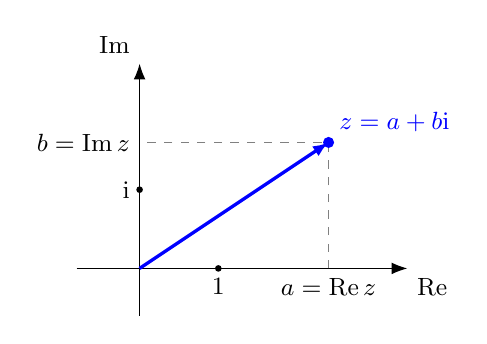
\begin{tikzpicture}[every node/.style={font=\small}, >={Latex[length=2mm]}]
	\draw[->] (-0.8,0) -- (3.4,0) node[below right] {$\mathrm{Re}$};
	\draw[->] (0,-0.6) -- (0,2.6) node[above left] {$\mathrm{Im}$};
	\draw[dashed, gray] (2.4,0) -- (2.4,1.6) -- (0,1.6);
	\draw[->, blue, very thick] (0,0) -- (2.4,1.6) node[above right] {$z=a+b\mathrm{i}$};
	\fill[blue] (2.4,1.6) circle (2pt);
	\node[below] at (2.4,0) {$a=\mathrm{Re}\,z$};
	\node[left] at (0,1.6) {$b=\mathrm{Im}\,z$};
	\fill (1,0) circle (1.2pt) node[below] {$1$};
	\fill (0,1) circle (1.2pt) node[left] {$\mathrm{i}$};
\end{tikzpicture}
\end{document}
